%%%%%%%%%%%%%%%%%%%%%%%%%%%%%%%%%%%%%%%%%
% Maggi Memoir Thesis
% XeLaTeX Template
% Version 1.0 (22/12/13)
%
% This template has been downloaded from:
% http://www.LaTeXTemplates.com
%
% Original authors:
% Federico Maggi (fede@maggi.cc) with extensive modifications by:
% Vel (vel@latextemplates.com)
%
% License:
% CC BY-NC-SA 3.0 (http://creativecommons.org/licenses/by-nc-sa/3.0/)
%
% Important notes:
% This template needs to be compiled with XeLaTeX.
%
% Most of the document content and packages are specified within structure.tex
% so if you need to make modifications to the template have a look there first!
%
% This template uses several fonts that are not available on most operating 
% systems by default. These are: Adobe Caslon Pro, Envy Code R and 
% Optima Regular. You will either need to obtain these and install them on your
% system or change them to different fonts. Simply go to the Fonts block just
% below here and modify their names to other fonts. You can also comment them 
% out completely to use the default LaTeX font.
%
%%%%%%%%%%%%%%%%%%%%%%%%%%%%%%%%%%%%%%%%%

%----------------------------------------------------------------------------------------
%	PACKAGES AND OTHER DOCUMENT CONFIGURATIONS
%----------------------------------------------------------------------------------------

\documentclass[10pt,showtrims,a4paper,twoside]{memoir} % Change font size here (allowable values are 9pt-12pt), change the paper size, specify one or two sided printing and specify whether to show trimming lines

%----------------------------------------------------------------------------------------
%	VARIOUS REQUIRED PACKAGES AND CONFIGURATIONS
%----------------------------------------------------------------------------------------

\XeTeXinputencoding latin1
\usepackage[T1]{fontenc} % Support for more character glyphs
\usepackage[round]{natbib}\citeindextrue % Round brackets around citations, change to square for square brackets
\usepackage{graphicx} % Required to include images
\usepackage{color} % Required for custom colors
\usepackage{amsmath,amssymb,theorem} % Math packages
\usepackage{listings} % Required for including snippets of code
\usepackage{booktabs} % Required for better horizontal rules in tables
\usepackage{xspace} % Provides the ability to use an intelligent space which is used in \institution and \department
\usepackage[printonlyused,withpage]{acronym} % Include a list of acronyms
\usepackage{rotating} % Allows tables and figures to be rotated
\usepackage{hyperref} % Required for links and changing link options
\usepackage{fontspec} % Required for specifying custom fonts in XeTeX
\usepackage{microtype} % Slightly tweak font spacing for aesthetics

\hypersetup{colorlinks, breaklinks, linkcolor=black,citecolor=black,filecolor=black,urlcolor=black} % Set up hyperlinks including colors for references, urls and citations

%\definecolor{c64}{rgb}{.063,0,.612} % Example color definition, the color can be used with the \color{name} command

\makeatletter
\renewcommand{\fnum@figure}{\textsc{\figurename~\thefigure}} % Make the "Figure 1.1" text in small caps
\makeatother

%----------------------------------------------------------------------------------------
%	PAGE LAYOUT
%----------------------------------------------------------------------------------------

% The memoir class used in this template contains the ability to set the stock paper size and the trimmed size independently. It also has the ability to show trim lines showing where stock paper should be trimmed to get the final book size. This can all be a bit confusing so please see the memoir class documentation for more information.

% By default, the paper size is a4paper which is 29.7cm × 21cm. To change this, simply change "a4paper" in the \documentclass[a4paper,...]{memoir} command in thesis.tex to another size such as "letterpaper".
% By default, the trimmed size is 24cm x 17cm and trim lines are shown. To remove trim lines, simply remove "showtrims" from the \documentclass[showtrims,...]{memoir} command in thesis.tex. The size of the trimmed content is set with the \settrimmedsize{}{} command below.
% If you wish to remove trims and set the content to fit the paper size (i.e. no trimming at all), all you have to do is remove "showtrims" as above and comment out the \settrimmedsize{}{} command below.

%\setstocksize{24cm}{17cm} % Uncomment to manually set the stock size and override the setting in \documentclass
\settrimmedsize{24cm}{17cm}{*} % Change the trimmed area size or comment out this line entirely to fit the content to the paper size without trimming
\setlrmarginsandblock{37.125mm}{*}{0.9} % The first bracket specifies the spine margin, the second the edge margin and the third the ratio of the spine to the edge. Only one or two values are required and the remaining one(s) can be a star (*) to specify it is not needed. By default the edge margin is 10% smaller and 
\setulmarginsandblock{37.125mm}{*}{*} % The first bracket specifies the upper margin, the second the lower margin and the third the ratio of the upper to the lower. Only one or two values are required and the remaining one(s) can be a star (*) to specify it is not needed.
\setmarginnotes{17pt}{51pt}{\onelineskip} % The size of marginal notes, the three values in curly brackets are \marginparsep, \marginparwidth and \marginparpush
\setheadfoot{\onelineskip}{2\onelineskip} % Sets the space available for the header and footer
\setheaderspaces{*}{2\onelineskip}{*} % Sets the spacing above and below the header
\setlength{\trimtop}{0pt} % Sets the spacing above the trimmed area, i.e. moved the trimmed area down the page if positive

% Comment the two lines below to reverse the position of the trimmed content on the stock paper, i.e. odd pages will have content on the right side instead of the left and even pages will have content on the left side instead of the right
\setlength{\trimedge}{\stockwidth}
\addtolength{\trimedge}{-\paperwidth}

\checkandfixthelayout % Makes sure your specifications are correct and implements them in the document

%----------------------------------------------------------------------------------------
%	CHAPTER HEADING STYLE
%----------------------------------------------------------------------------------------

\makeatletter
\makechapterstyle{thesis}{
\renewcommand{\chapternamenum}{}
\setlength{\beforechapskip}{0pt}
\setlength{\midchapskip}{0pt}
\setlength{\afterchapskip}{0pt}
\renewcommand{\chapnamefont}{\LARGE}
\renewcommand{\chapnumfont}{\chapnamefont}
\renewcommand{\chaptitlefont}{\chapnamefont}
\renewcommand{\printchapternum}{}
\renewcommand{\afterchapternum}{}
\renewcommand{\printchaptername}{}
\renewcommand{\afterchaptertitle}{\chapnumfont\hfill\thechapter\\\vspace*{-.3cm}\hrulefill\vspace*{6cm}\\}
}
\makeatother

%----------------------------------------------------------------------------------------
%	TABLE OF CONTENTS DEPTH
%----------------------------------------------------------------------------------------

\maxsecnumdepth{subsubsection}
\maxtocdepth{subsection}

%----------------------------------------------------------------------------------------
%	MATH THEOREM DEFINITIONS
%----------------------------------------------------------------------------------------

\theoremstyle{plain}
\newtheorem{thm}{Theorem}[section] % Defines the theorem environment
\newtheorem{prop}[thm]{Proposition} % Defines the proposition environment
\newtheorem{proof}{Proof}[section] % Defines the proof environment
\newtheorem{definition}{Definition}[section] % Defines the definition environment
\newtheorem{example}{Example}[section] % Defines the example environment
\newtheorem{rem}{Remark} % Defines the remark environment
\newtheorem{note}{Note}[section] % Defines the note environment

%----------------------------------------------------------------------------------------
%	CODE SNIPPET CONFIGURATION
%----------------------------------------------------------------------------------------

\lstset{
  basicstyle=\ttfamily\small,
  basewidth=0.55em,
  showstringspaces=false,
  numbers=left,
  numberstyle=\tiny,
  numbersep=2.5pt,
  keywordstyle=\bfseries\ttfamily,
  breaklines=true
}
% Examples of list environments for different programming languages, you will likely need to specify your own
\lstnewenvironment{pseudoc}{\lstset{frame=lines,language=C,mathescape=true}}{}
\lstnewenvironment{logs}{\lstset{frame=lines,basicstyle=\footnotesize\ttfamily,numbers=none}}{}
\lstnewenvironment{cc}{\lstset{frame=lines,language=C}}{}
\lstnewenvironment{c64}{\lstset{backgroundcolor=\color{c64},basewidth=0.65em,basicstyle=\commodoreface\color{c64light},numbers=none,framerule=10pt,rulecolor=\color{c64light},frame=tb,framexbottommargin=30pt}}{}
\lstnewenvironment{html}{\lstset{frame=lines,language=html,numbers=none}}{}
\lstnewenvironment{pseudo}{\lstset{frame=lines,mathescape=true,morekeywords={learn_string_domain, save_model}}}{}
\lstnewenvironment{pseudoctiny}{\lstset{language=C,mathescape=true,basicstyle=\tiny\sffamily}}{}
\lstnewenvironment{cctiny}{\lstset{language=C,basicstyle=\tiny\sffamily}}{}
\lstnewenvironment{pseudotiny}{\lstset{mathescape=true,basicstyle=\tiny\sffamily}}{} % Include the file containing the code defining the structure and style of the document

%------------------------------------------------
% Thesis Information

\title{Integrated Detection of Anomalous Behavior of Computer Infrastructures} % Thesis title

\author{Federico Maggi} % Author name

\date{December 2013} % The date

\newcommand{\institution}{University of California\xspace} % University/institution name

\newcommand{\department}{Department of Computer Science\xspace} % Department name

%------------------------------------------------
% Fonts

\defaultfontfeatures{Mapping=tex-text}
\setromanfont[Ligatures={Common}]{Adobe Caslon Pro} % Normal document font
\setmonofont[Scale=0.8]{Envy Code R} % Mono spaced font (\texttt{})
\setsansfont[Scale=0.9]{Optima Regular} % Sans-serif font (\textsf{})

\renewcommand*{\acffont}[1]{{\normalsize\itshape #1}} % Font style for the acronym text (e.g. Do It Yourself)
\renewcommand*{\acfsfont}[1]{{\normalsize\upshape #1}} % Font style for the acronym in bracket (e.g. (DIY))

%------------------------------------------------
% Hyphenations

\hyphenation{a-no-ma-lous a-no-ma-ly amounts breaches} % Specify custom hyphenation points in words with dashes where you would like hyphenation to occur, or alternatively, don't put any dashes in a word to stop hyphenation altogether

%----------------------------------------------------------------------------------------
%	TITLE PAGE
%----------------------------------------------------------------------------------------

\renewcommand{\maketitlehooka}{
\centering

\includegraphics[width=2.5cm]{Figures/polimi-logo}\\[.5cm] % Institution logo
\institution\\ % Print institution name
\emph{\department}\\[.2cm] % Print department name
DOTTORATO DI RICERCA IN INGEGNERIA DELL'INFORMAZIONE % Degree or other information
\par
\hrulefill
\vfill}
\renewcommand{\maketitlehookb}{\vfill}
\renewcommand{\maketitlehookc}{
\vfill
\begin{flushleft}
Advisor:\\
\textbf{Prof. Stefano Zanero}\\[.3cm] % Advisor's/supervisor's name
Tutor:\\
\textbf{Prof. Letizia Tanca}\\[.3cm] % Tutor's name
Supervisor of the Doctoral Program:\\
\textbf{Prof. Patrizio Colaneri} % Doctoral program supervisor's name
\end{flushleft}
\vfill}
\preauthor{\begin{flushright}Doctoral Dissertation of:\\\bfseries} % Text prior to the author name - right aligned and bold
\postauthor{\end{flushright}} % After the author name, stop right alignment

%----------------------------------------------------------------------------------------

\makeindex % Write an index file

\begin{document}

\begin{titlingpage}
\maketitle % Print the title page
\end{titlingpage}

\frontmatter % Use roman page numbering style (i, ii, iii, iv...) for the pre-content pages

%----------------------------------------------------------------------------------------
%	PREFACE
%----------------------------------------------------------------------------------------

\section*{Preface}
This thesis embraces all the efforts that I put during the last three years as a PhD student at Politecnico di Milano. I have been working under the supervision of Prof. S. Zanero and Prof. G. Serazzi, who is also the leader of the research group I am part of. In this time frame I had the wonderful opportunity of being ``initiated'' to research, which radically changed the way I look at things: I found my natural \emph{``thinking outside the box''} attitude --- that was probably well-hidden under a thick layer of lack-of-opportunities, I took part of very interesting joint works --- among which the year I spent at the Computer Security Laboratory at UC Santa Barbara is at the first place, and I discovered the Zen of my life.

My research is all about \emph{computers} and every other technology possibly related to them. Clearly, the way I look at computers has changed a bit since when I was seven. Still, I can remember me, typing on that \textsf{Commodore} 64 in front of a tube TV screen, trying to get that d---n routine written in \textsf{Basic} to work. I was just playing, obviously, but when I recently found a picture of me in front of that screen...it all became clear.

So, although my attempt of writing a program to authenticate myself was a little bit naive --- being limited to a print instruction up to that point apart, of course --- I thought \emph{``maybe I am not in the wrong place, and the fact that my research is still about security is a good sign''}!

Many years later, this work comes to life. There is a humongous amount of people that, directly or indirectly, have contributed to my research and, in particular, to this work. Since my first step into the lab, I will not, ever, be thankful enough to Stefano, who, despite my skepticism, convinced me to submit that application for the PhD program. For trusting me since the very first moment I am thankful to Prof. G. Serazzi as well, who has been always supportive. For hosting and supporting my research abroad I thank Prof. G. Vigna, Prof. C. Kruegel, and Prof. R. Kemmerer. Also, I wish to thank Prof. M. Matteucci for the great collaboration, Prof. I. Epifani for her insightful suggestions and Prof. H. Bos for the detailed review and the constructive comments.

On the colleagues-side of this acknowledgments I put all the fellows of Room 157, Guido, the crew of the seclab and, in particular, Wil with whom I shared all the pain of paper writing between Sept '08 and Jun '09.

On the friends-side of this list Lorenzo and Simona go first, for being our family.

I have tried to translate in simple words the infinite gratitude I have and will always have to Valentina and my parents for being my fixed point in my life. Obviously, I failed.

\begin{flushright}
\textsc{\theauthor}\\
Milano\\
September 2009
\end{flushright}

\cleartoverso % Force a break to an even page

%----------------------------------------------------------------------------------------
%	ABSTRACT
%----------------------------------------------------------------------------------------

\begin{abstract}
This dissertation details our research on anomaly detection techniques, that are central to several classic security-related tasks such as network monitoring, but it also have broader applications such as program behavior characterization or malware\index{malware} classification. In particular, we worked on anomaly detection from three different perspective, with the common goal of recognizing awkward activity on computer infrastructures. In fact, a computer system has several weak spots that must be protected to avoid attackers to take advantage of them. We focused on protecting the operating system, central to any computer, to avoid malicious code to subvert its normal activity. Secondly, we concentrated on protecting the web applications, which can be considered the modern, shared operating systems; because of their immense popularity, they have indeed become the most targeted entry point to violate a system. Last, we experimented with novel techniques with the aim of identifying related events (e.g., alerts reported by intrusion detection systems) to build new and more compact knowledge to detect malicious activity on large-scale systems.

Our contributions regarding host-based protection systems focus on characterizing a process' behavior through the system calls invoked into the kernel. In particular, we engineered and carefully tested different versions of a multi-model detection system using both stochastic and deterministic models to capture the features of the system calls during normal operation of the operating system. Besides demonstrating the effectiveness of our approaches, we confirmed that the use of finite-state, deterministic models allow to detect deviations from the process' control flow with the highest accuracy; however, our contribution combine this effectiveness with advanced models for the system calls' arguments resulting in a significantly decreased number of false alarms.

Our contributions regarding web-based protection systems focus on advanced training procedures to enable learning systems to perform well even in presence of changes in the web application source code --- particularly frequent in the Web 2.0 era. We also addressed data scarcity issues that is a real problem when deploying an anomaly detector to protect a new, never-used-before application. Both these issues dramatically decrease the detection capabilities of an intrusion detection system but can be effectively mitigated by adopting the techniques we propose.

Last, we investigated the use of different stochastic and fuzzy models to perform automatic alert correlation, which is as post processing step to intrusion detection. We proposed a fuzzy model that formally defines the errors that inevitably occur if time-based alert aggregation (i.e., two alerts are considered correlated if they are close in time) is used. This model allow to account for measurements errors and avoid false correlations due to delays, for instance, or incorrect parameter settings. In addition, we defined a model to describe the alert generation as a stochastic process and experimented with non-parametric statistical tests to define robust, zero-configuration correlation systems.

The aforementioned tools have been tested over different datasets --- that are thoroughly documented in this document --- and lead to interesting results.
\end{abstract}

\cleartoverso % Force a break to an even page

%----------------------------------------------------------------------------------------
%	TABLE OF CONTENTS
%----------------------------------------------------------------------------------------

\tableofcontents* % Print the table of contents

\cleartoverso % Force a break to an even page

%----------------------------------------------------------------------------------------
%	LIST OF FIGURES
%----------------------------------------------------------------------------------------

\listoffigures % Print the list of figures

\cleartoverso % Force a break to an even page

%----------------------------------------------------------------------------------------
%	LIST OF TABLES
%----------------------------------------------------------------------------------------

\listoftables % Print the list of tables

\cleartoverso % Force a break to an even page

%----------------------------------------------------------------------------------------
%	ACRONYMS
%----------------------------------------------------------------------------------------

\chapter{List of Acronyms}
\begin{acronym}\addtolength{\itemsep}{-\baselineskip}
  \acro{AIC}{Akaike Information Criterion}
  \acro{ARMA}{Auto Regressive Moving Average}
  \acro{ARMAX}{Auto Regressive Moving Average eXogenous}
  \acro{ARX}{Auto Regressive eXogenous}
  \acro{AR}{Auto Regressive}
  \acro{ARR}{Alert Reduction Rate}
  \acro{ANSI}{American National Standard Institute}
  \acro{ASCII}{American Standard for Information Interxchange}
  \acro{BIC}{Bayesian Information Criterion}
  \acro{BMU}{Best Matching Unit}
  \acro{BSM}{Basic Security Module}
  \acro{CDF}{Cumulative Density Function}
  \acro{CDX}{Cyber Defense eXercise}
  \acro{CIA}{Confidentially Integrity Availability}
  \acro{CIDS}{Collaborative IDS}
  \acro{CPU}{Central Processing Unit}
  \acro{CSV}{Comma Separated Values}
  \acro{CTF}{Capture The Flag}
  \acro{DAG}{Direct Acyclic Graph}
  \acro{DARPA}{Defense Advanced Research Projects Agency}
  \acro{DB}{DataBase}
  \acro{DBMS}{DataBase Management System}
  \acro{DIDS}{Distributed IDS}
  \acro{DNS}{Domain Name System}
  \acro{DOM}{Document Object Model}
  \acro{DoS}{Denial of Service}
  \acro{DR}{Detection Rate}
  \acro{DTD}{Document Type Definition}
  \acro{ED}{Elementary Detector}
  \acro{ELF}{Executable Linux Format}
  \acro{FN}{False Negative}
  \acro{FNR}{False Negative Rate}
  \acro{FPR}{False Positive Rate}
  \acro{FP}{False Positive}
  \acro{FSA}{Finite State Automaton}
  \acro{FTP}{File Transfer Protocol}
  \acro{GCI}{Granger Causality Index}
  \acro{GCT}{Granger Causality Test}
  \acro{HIDS}{Host-based Intrusion Detection System}
  \acro{HMM}{Hidden Markov Model}
  \acro{HTML}{HyperText Markup Language}
  \acro{HTTP}{HyperText Transfer Protocol}
  \acro{ICD}{Idealized Character Distribution}
  \acro{IDEVAL}{Intrusion Detection eVALuation}
  \acro{IDMEF}{Intrusion Detection Message Exchange Format}
  \acro{IDS}{Intrusion Detection System}
  \acro{IDWG}{Intrusion Detection Working Group}
  \acro{ID}{Intrusion Detection}
  \acro{IETF}{Internet Engineering Task Force}
  \acro{IODEF}{Incident Object Description and Interchange Format}
  \acro{IPS}{Intrusion Protection System}
  \acro{ISP}{Internet Service Provider}
  \acro{IP}{Internet Protocol}
  \acro{IR}{Information Retrieval}
  \acro{IRC}{Internet Relay Chat}
  \acro{ISS}{Internet Security Systems}
  \acro{JSON}{JavaScript Object Notation}
  \acro{KBS}{Knowledge Base System}
  \acro{KS}{Kolmogorov-Smirnoff}
  \acro{LARIAT}{Lincoln Adaptable Real-time Information Assurance Testbed}
  \acro{LERAD}{Learning Rules for Anomaly Detection}
  \acro{LL}{Lincoln Laboratory}
  \acro{MDL}{Minimum Description Length}
  \acro{MIT}{Massachusetts Institute of Technology}
  \acro{ML}{Maximum Likelihood}
  \acro{MTU}{Maximum Transfer Unit}
  \acro{NIDES}{Next-generation Intrusion Detection Expert System}
  \acro{NIDS}{Network-based Intrusion Detection System}
  \acro{NNID}{Neural Network Intrusion Detection}
  \acro{NSTISSC}{National Security Telecomm. and Information Systems Sec. Committee}
  \acro{NTP}{Network Time Protocol}
  \acro{PC}{Program Counter}
  \acro{PDF}{Probability Density Function}
  \acro{PHAD}{Packet Header Anomaly Detection}
  \acro{PHP}{PHP Hypertext Preprocessor}
  \acro{PID}{Process IDentifier}
  \acro{ROC}{Receiving Operating Characteristic}
  \acro{SADE}{Syscall Sequence Arguments Anomaly Detection Engine}
  \acro{SDEE}{Security Device Event Exchange}
  \acro{SMTP}{Simple Message Transfer Protocol}
  \acro{SOM}{Self Organizing Map}
  \acro{SQL}{Structured Query Language}  
  \acro{SRI}{Stanford Research Institute}
  \acro{SSH}{Secure SHell}
  \acro{STATL}{State Transition Analysis Technique Language}
  \acro{SVN}{SubVersioN}
  \acro{SYN}{SYNchronize}
  \acro{TCP}{Trasmission Control Protocol}
  \acro{TF}{Truth File}
  \acro{TN}{True Negative}
  \acro{TNR}{True Negative Rate}
  \acro{TOS}{Type Of Service}
  \acro{TP}{True Positive}
  \acro{TTL}{Time To Live}
  \acro{UCSB}{University of California Santa Barbara}
  \acro{ULISSE}{Unsupervised Learning IDS with 2-Stages Engine}
  \acro{UDP}{User Datagram Protocol}
  \acro{UML}{Unified Modeling Language}
  \acro{URL}{Uniform Resource Locator}
  \acro{VPN}{Virtual Private Network}
  \acro{XML}{eXtensible Markup Language}
  \acro{XSD}{XML Schema Definition}
  \acro{XSS}{Cross-Site Scripting}
\end{acronym} % Include a List of Acronyms section using acronyms.tex where they are defined

\cleartoverso % Force a break to an even page

%----------------------------------------------------------------------------------------
%	COLOPHON
%----------------------------------------------------------------------------------------

\thispagestyle{empty} % Remove all headers and footers from this page

\vspace*{2em}
\renewcommand{\abstractname}{Colophon}
\begin{abstract}
This document was typeset using the \textsf{XeTeX} typesetting system created by the Non-Roman Script Initiative and the memoir class created by Peter Wilson. The body text is set 10pt with~Adobe Caslon Pro. Other fonts include \texttt{Envy Code R}, \textsf{Optima Regular} and. Most of the drawings are typeset using the \textsf{TikZ/PGF} packages by Till Tantau.
\end{abstract}
\vfill

%----------------------------------------------------------------------------------------
%	CONTENT CHAPTERS
%----------------------------------------------------------------------------------------

\mainmatter % Begin numeric (1,2,3...) page numbering

\chapterstyle{thesis} % Change the style of the Chapter header to that defined in structure.tex

\pagestyle{Ruled} % Include the chapter/section in the header along with a horizontal rule underneath

\chapter{Introduction}
\label{introduction}

Network connected devices such as personal computers, mobile phones, or gaming consoles are nowadays enjoying immense popularity. In parallel, the Web and the humongous amount of services it offers have certainly became the most ubiquitous tools of all the times. \textsf{Facebook} counts more than 250 millions active users of which 65 millions are using it on mobile devices; not to mention that more than 1 billion photos are uploaded to the site \emph{each   month}~\citep{facebook-stats}. And this is just one, popular website. One year ago, \textsf{Google} estimated that the approximate number of unique \acp{URL}\index{URL} is 1 trillion~\citep{google-is-big}, while \texttt{YouTube} has stocked more than 70 million videos as of March 2008, with 112,486,327 views just on the most popular video as of January 2009~\citep{social-media-stats}. And people from all over the world inundate the Web with more than 3 million tweets \emph{per day}. Not only the Web 2.0 has became predominant; in fact, thinking that on December 1990 the Internet was made of \emph{one} site and today it counts more than 100 million sites is just astonishing~\citep{internet-timeline}.

The Internet and the Web are huge~\citep{inetworldstats}. The relevant fact, however, is that they both became the most advanced workplace. Almost every industry connected its own network to the Internet and relies on these infrastructures for a vast majority of transactions; most of the time monetary transactions. As an example, every year \textsf{Google} looses approximately 110 millions of US Dollars in ignored ads because of the \emph{``I'm feeling lucky''} button. The scary part is that, during their daily work activities, people typically pay poor or no attention at all to the risks that derive from exchanging any kind of information over such a complex, interconnected infrastructure. This is demonstrated by the effectiveness of social engineering~\citep{deception} scams carried over the Internet or the phone~\citep{social-engineering-fundamentals}. Recall that 76\% of the phishing is related to finance. Now, compare this landscape to what the most famous security quote states.

\begin{quotation}
  ``The only truly secure computer is one buried in concrete, with the   power turned off and the network cable cut''.
   ---\emph{Anonymous}
\end{quotation}

In fact, the Internet is all but a safe place~\citep{whid}, with more than 1,250 \emph{known} data breaches between 2005 and 2009 \citep{data-breaches-chronology} and an estimate of 263,470,869 records stolen by intruders. One may wonder why the advance of research in computer security and the increased awareness of governments and public institutions are still not capable of avoiding such incidents. Besides the fact that the aforementioned numbers would be order of magnitude higher in absence of countermeasures, todays' security issues are, basically, caused by the combination of two phenomena: the high amount of software vulnerabilities and the effectiveness of todays' exploitation strategy.

\begin{description}
\item[software flaws] --- (un)surprisingly, software is affected by   vulnerabilities. Incidentally, tools that have to do with the Web,   namely, browsers and 3\textsuperscript{rd}-party extensions, and web   applications, are the most vulnerable ones. For instance, in 2008,   \textsf{Secunia} reported around 115 security vulnerabilities for   \textsf{Mozilla Firefox}, 366 for \textsf{Internet Explorer}'s   \textsf{ActiveX}~\citep{secunia2008}. Office suites and e-mail   clients, that are certainly the must-have-installed tool   on every workstation, hold the second position~\citep{sans20}.
  
\item[massification of attacks] --- in parallel to the explosion of   the Web 2.0, attackers and the underground economy have quickly   learned that a sweep of exploits run against \emph{every} reachable   host have more chances to find a vulnerable target and, thus, is   much more profitable compared to a single effort to break into a   high-value, well-protected machine.
\end{description}

These circumstances have initiated a vicious circle that provides the attackers with a very large pool of vulnerable targets. Vulnerable client hosts are compromised to ensure virtually unlimited bandwidth and computational resources to attackers, while server side applications are violated to host malicious code used to infect client visitors. And so forth. An old fashioned attacker would have violated a single site using all the resources available, stolen data and sold it to the underground market. Instead, a modern attacker adopts a ``vampire'' approach and exploit client-side software vulnerabilities to take (remote) control of million hosts. In the past the diffusion of malicious code such as viruses was sustained by sharing of infected, cracked software through floppy or compact disks; nowadays, the Web offers unlimited, public storage to attackers that deploy their exploit on compromised websites.

Thus, not only the type of vulnerabilities has changed, posing virtually every interconnected device at risk. The exploitation strategy created new types of threats that take advantage of classic malicious code patterns but in a new, extensive, and tremendously effective way.

\section{Todays' Security Threats}
\label{introduction:motivation} Every year, new threats are discovered and attacker take advantage of them until effective countermeasures are found. Then, new threats are discovered, and so forth. \textsf{Symantec} quantifies the amount of new malicious code threats to be 1,656,227 as of 2008 \citep{symantec_threat_report_2009}, 624,267 one year earlier and only 20,547 in 2002. Thus, countermeasures must advance at least with the same grow rate. In addition:

\begin{figure}[t]
  \centering
  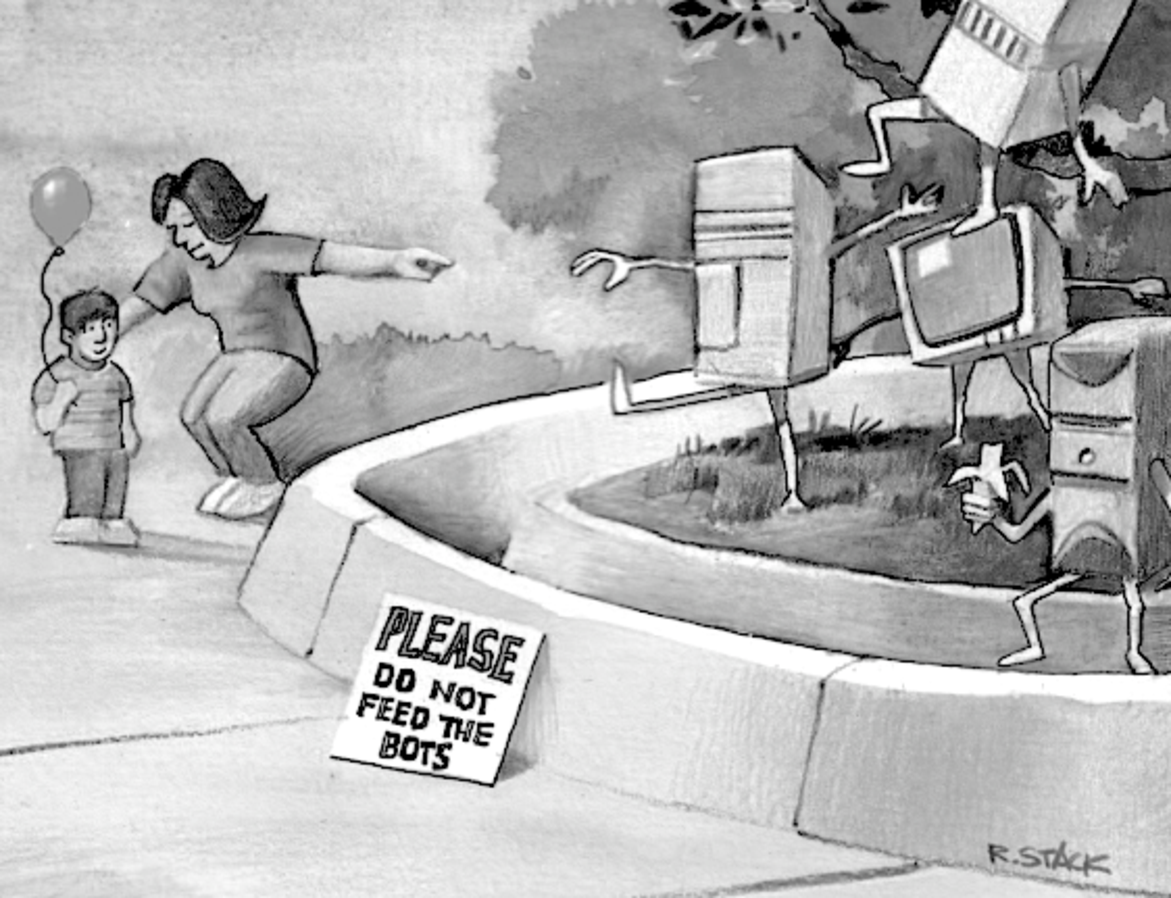
\includegraphics[width=\textwidth]{Figures/bots.pdf}
  \caption{Illustration taken from~\citep{holz} and \copyright 2005 IEEE. Authorized license limited to \institution.}
  \label{fig:bots}
\end{figure}

\begin{quotation}
  [...] the current threat landscape --- such as the increasing complexity and sophistication of attacks, the evolution of attackers
and attack patterns, and malicious activities being pushed to emerging countries --- show not just the benefits of, but also the need for increased cooperation among security companies, governments, academics, and other organizations and individuals to combat these changes~\citep{symantec_threat_report_2009}.
\end{quotation}

Todays' underground economy run a very proficient market: everyone can buy credit card information for as low as \$0.06--\$30, full identities for just \$0.70--\$60 or rent a scam hosting solution for \$3--\$40 per week plus \$2-\$20 for the design~\citep{symantec_threat_report_2009}.

The main underlying technology actually employs a classic type of software called \emph{bot} (jargon for \emph{robot}), which is not malicious \emph{per s\'e}, but is used to remotely control a network of compromised hosts, called \emph{botnet}~\citep{holz}. Remote commands can be of any type and typically include launching an attack, starting a phishing or spam campaign, or even updating to the latest version of the bot software by downloading the binary code from a host controlled by the attackers (usually called \emph{bot master})~\citep{torpig}. The exchange good has now become the botnet infrastructure itself rather than the data that can be stolen or the spam that can be sent. These are mere outputs of todays' most popular service offered for rent by the underground economy.

\subsection{The Role of Intrusion Detection}
\label{introduction:motivation:ids-role}
The aforementioned, dramatic big picture may lead to think that the malicious software will eventually proliferate at every host of the Internet and no effective remediation exists. However, a more careful analysis reveals that, despite the complexity of this scenario, the problems that must be solved by a security infrastructure can be decomposed into relatively simple tasks that, surprisingly, may already have a solution. Let us look at an example.

\begin{example}
This is how a sample exploitation can be structured:
\begin{description}
\item [injection] --- a malicious request is sent to the vulnerable web application with the goal of corrupting all the responses sent to legitimate clients from that moment on. For instance, more than one releases of the popular \textsf{WordPress} blog application are vulnerable to injection attacks\footnote{http://secunia.com/advisories/23595} that allow an attacker to permanently include arbitrary content to the pages. Typically, such an arbitrary content is malicious code (e.g., JavaScript, VBSCrip, ActionScript, ActiveX) that, every time a legitimate user requests the infected page, executes on the client host.
\item [infection] --- Assuming that the compromised site is frequently accessed --- this might be the realistic case of the \textsf{WordPress}-powered \textsf{ZDNet} news blog\footnote{http://wordpress.org/showcase/zdnet/} --- a significant amount of clients visit it. Due to the high popularity of vulnerable browsers and plug-ins, the client may run \textsf{Internet Explorer} --- that is the most popular --- or an outdated release of \textsf{Firefox} on \textsf{Windows}. This create the perfect circumstances for the malicious page to successfully execute. In the best case, it may download a virus or a generic malware from a website under control of the attacker, so infecting the machine. In the worst case, this code may also exploit specific browser vulnerabilities and execute in privileged mode.
\item [control \& use] --- The malicious code just download installs and hides itself onto the victim's computer, which has just joined a botnet. As part of it, the client host can be remotely controlled by the attackers who can, for instance, rent it, use its bandwidth and computational power along with other computers to run a distributed \ac{DoS} attack. Also, the host can be used to automatically perform the same attacks described above against other vulnerable web applications. And so forth. \end{description}
\end{example}

This simple yet quite realistic example shows the various kinds of malicious activity that are generated during a typical drive-by exploitation. It also shows its requirements and assumptions that must hold to guarantee success. More precisely, we can recognize:

\begin{description}
\item[network activity] --- clearly, the whole interaction relies on a network connection over the Internet: the \ac{HTTP} connections used, for instance, to download the malicious code as well as to launch the injection attack used to compromise the web server.
\item[host activity] --- similarly to every other type of attack against an application, when the client-side code executes, the browser (or one of its extension plug-ins) is forced to behave improperly. If the malicious code executes till completion the attack succeeds and the host is infected. This happens only if the platform, operating system, and browser all match the requirements assumed by the exploit designer. For instance, the attack may succeed on \textsf{Windows} and not on \textsf{Mac OS X}, although the vulnerable version of, say, \textsf{Firefox} is the same on both the hosts.
\item[HTTP traffic] --- in order to exploit the vulnerability of the web application, the attacking client must generate malicious \ac{HTTP} requests. For instance, in the case of an \ac{SQL} injection --- that is the second most common vulnerability in a web application --- instead of a regular

\begin{logs}
GET /index.php?username=myuser
\end{logs}
  
\noindent the web server might be forced to process a

\begin{logs}
GET /index.php?username=' OR 'x'='x'--\&content=<script src="evil.com/code.js">
\end{logs}

\noindent that causes the \texttt{index.php} page to behave improperly.
\end{description}

It is now clear that protection mechanisms that analyze the network traffic, the activity of the client's operating system, the web server's \ac{HTTP} logs, or any combination of the three, have chances of recognizing that something malicious is happening in the network. For instance, if the \ac{ISP} network adopt \textsf{Snort}, a lightweight \ac{IDS} that analyzes the network traffic for known attack patterns, could block all the packets marked as suspicious. This would prevent, for instance, the \ac{SQL} injection to reach the web application. A similar protection level can be achieved by using other tools such as \textsf{ModSecurity} \citep{ristic:mod_security}. One of the problems that may arise with these classic, widely adopted solutions is if a zero day\index{0-day} attack is used. A zero day attack or threat exploits a vulnerability that is unknown to the public, undisclosed to the software vendor, or a fix is not available; thus, protection mechanisms that merely blacklist known malicious activity immediately become ineffective. In a similar vein, if the client is protected by an anti-virus, the infection phase can be blocked. However, this countermeasure is once again successful only if the anti-virus is capable of recognizing the malicious code, which assumes that the code is known to be malicious.

Ideally, an effective and comprehensive countermeasure can be achieved if all the protection tools involved (e.g., client-side, server-side, network-side) can collaborate together. For instance, if a website is publicly reported to be malicious, a client-side protection tool should block all the content downloaded from that particular website. This is only a simple example.

Thus, countermeasures against todays' threats already exist but are subject to at least two drawbacks:

\begin{itemize}
\item they offer protection only against known threats. To be effective we must assume that all the hostile traffic can be enumerated, which is clearly an impossible task.

\begin{quotation}
Why is ``Enumerating Badness'' a dumb idea? It's a dumb idea because sometime around 1992 the amount of Badness in the Internet began to vastly outweigh the amount of Goodness. For every harmless, legitimate, application, there are dozens or hundreds of pieces of malware, worm tests, exploits, or viral code. Examine a typical antivirus package and you'll see it knows about 75,000+ viruses that might infect your machine. Compare that to the legitimate 30 or so apps that I've installed on my machine, and you can see it's rather dumb to try to track 75,000 pieces of Badness when even a simpleton could track 30 pieces of Goodness~\citep{ranum-myths}.
\end{quotation}

\item they lack of cooperation, which is crucial to detect global and slow attacks.
\end{itemize}

This said, we conclude that classic approaches such as dynamic and static code analysis and \ac{IDS} already offer good protection but industry and research should move toward methods that require little or no knowledge. In this work, we indeed focus on the so called anomaly-based approaches, i.e., those that attempt to recognize the threats by detecting any variation from a system's normal operation, rather than looking for signs of known-to-be-malicious activity.

\section{Original Contributions}
\label{introduction:contributions} Our main research area is \ac{ID}. In particular, we focus on anomaly-based approaches to detect malicious activities. Since todays' threats are complex, a single point of inspection is not effective. A more comprehensive monitoring system is more desirable to protect both the network, the applications running on a certain host, and the web applications (that are particularly exposed due to the immense popularity of the Web). Our contributions focus on the mitigation of both host-based and web-based attacks, along with two techniques to correlate alerts from hybrid sensors.

\subsection{Host-based Anomaly Detection} Typical malicious processes can be detected by modeling the characteristics (e.g., type of arguments, sequences) of the system calls executed by the kernel, and by flagging unexpected deviations as attacks. Regarding this type of approaches, our contributions focus on hybrid models to accurately characterize the behavior of a binary application. In particular:

\begin{itemize}
\item we enhanced, re-engineered, and evaluated a novel tool for modeling the normal activity of the Linux 2.6 kernel. Compared to other existing solutions, our system shows better detection capabilities and good contextualization of the alerts reported.
\item We engineered and evaluated an \ac{IDS} to demonstrate that the combined use of (1) deterministic models to characterize a process' control flow and (2) stochastic models to capture normal features of the data flow, lead to better detection accuracy. Compared to the existing deterministic and stochastic approaches separately, our system shows better accuracy, with almost zero false positives.
\item We adapted our techniques for forensics investigation. By running experiments on real-world data and attacks, we show that our system is able to detect hidden tamper evidence although sophisticated anti-forensics tools (e.g., userland process execution) have been used.
\end{itemize}

\subsection{Web-based Anomaly Detection} Attempts of compromising a web application can be detected by modeling the characteristics (e.g., parameter values, character distributions, session content) of the \ac{HTTP}\index{HTTP} messages exchanged between servers and clients during normal operation. This approach can detect virtually any attempt of tampering with \ac{HTTP}\index{HTTP} messages, which is assumed to be evidence of attack. In this research field, our contributions focus on training data scarcity issues along with the problems that arise when an application changes its legit behavior. In particular:

\begin{itemize}
\item we contributed to the development of a system that learns the legit behavior of a web application. Such a behavior is defined by means of features extracted from 1) HTTP requests, 2) HTTP responses, 3) SQL queries to the underlying database, if any. Each feature is extracted and learned by using different models, some of which are improvements over well-known approaches and some others are original. The main contribution of this work is the \emph{combination} of database query models with HTTP-based models. The resulting system has been validated through preliminary experiments that shown very high accuracy.
\item we developed a technique to automatically detect legit changes in web applications with the goal of suppressing the large amount of false detections due to code upgrades, frequent in todays' web applications. We run experiments on real-world data to show that our simple but very effective approach accurately predict changes in web applications and can distinguish good \emph{vs.} malicious changes (i.e., attacks).
\item We designed and evaluated a machine learning technique to aggregate \ac{IDS} models with the goal of ensuring good detection accuracy even in case of scarce training data available. Our approach relies on clustering techniques and nearest-neighbor search to look-up well-trained models used to replace under-trained ones that are prone to overfitting and thus false detections. Experiments on real-world data have shown that almost every false alert due to overfitting is avoided with as low as 32-64 training samples per model.
\end{itemize}

Although these techniques have been developed on top of a web-based anomaly detector, they are sufficiently generic to be easily adapted to other systems using learning approaches.

\subsection{Alert Correlation} \ac{IDS} alerts are usually post-processed to generate compact reports and eliminate redundant, meaningless, or false detections. In this research field, our contributions focus on unsupervised techniques applied to aggregate and correlate alert events with the goal of reducing the effort of the security officer. In particular:

\begin{itemize}
\item We developed and tested an approach that accounts for the common measurement errors (e.g., delays and uncertainties) that occur in the alert generation process. Our approach exploits fuzzy metrics both to model errors and to construct an alert aggregation criterion based on distance in time. This technique has been show to be more robust compared to classic time-distance based aggregation metrics.
\item We designed and tested a prototype that models the alert generation process as a stochastic process. This setting allowed us to construct a simple, non-parametric hypothesis test that can detect whether two alert streams are correlated or not. Besides its simplicity, the advantage of our approach is to not requiring any parameter.
\end{itemize}

The aforementioned results have been published in the proceedings of international conferences and international journals. % Include the introduction chapter
\chapter{A Chapter of Examples}
\label{chapter1}

\section{A Table}

\begin{table}[h]
\centering
\begin{tabular}{rcc}
\toprule \emph{Feature} & \textsc{Misuse-based} &
\textsc{Anomaly-based}\\
    
\midrule Modeled activity: & Malicious & Normal\\
Detection method: & Matching & Deviation\\
Threats detected: & Known & Any\\
False negatives: & High & Low\\
False positives: & Low & High\\
Maintenance cost: & High & Low\\
Attack desc.: & Accurate & Absent\\
System design: & Easy & Difficult\\
\bottomrule
\end{tabular}
\caption[Duality between misuse- and anomaly-based intrusion detection techniques.]{Duality between misuse- and anomaly-based intrusion detection techniques. Note that, an anomaly-based \ac{IDS} can detect ``Any'' threat, under the assumption that an attack always generates a deviation in the modeled activity.}
\label{tab:misuse-vs-anomaly}
\end{table}

%------------------------------------------------

\section{Code}

\begin{pseudoc}
  /* ... */ cd['<'] = {0.1, 0.11} cd['a'] = {0.01, 0.2} cd['b'] =
  {0.13, 0.23} /* ... */

  b = decode(arg3_value);
  
  if ( !(cd['c'][0] < count('c', b) < cd['c'][1]) ||\
       !(cd['<'][0] < count('<', b) < cd['<'][1]) ||\
       ... || ...)  fire_alert("Anomalous content detected!");
  /* ... */
\end{pseudoc}

%------------------------------------------------

\section{A Sideways Table}

\clearpage
\begin{sidewaystable}
\renewcommand{\arraystretch}{1.5} \centering
\begin{tabular}{rcccccc}
\toprule \textsc{Approach} & \textsc{Time} & \textsc{Header} &
\textsc{Payload} & \textsc{Stochastic} & \textsc{Determ.} & \textsc{Clustering}\\
\midrule \citep{phad} & & $\bullet$ & & & & $\bullet$ \\
\citep{kruegel:sac2002:anomaly} & & $\bullet$ & $\bullet$ & $\bullet$ & & \\
\citep{protocolanom} & & $\bullet$ & & $\bullet$ & $\bullet$ & \\
\citep{ramadas} & & & $\bullet$ & & & $\bullet$ \\
\citep{rules-payl} & $\bullet$ & & $\bullet$ & & $\bullet$ & \\
\citep{zanero-savaresi} & & $\bullet$ & $\bullet$ & & & $\bullet$ \\
\citep{wang:raid2004:payl} & & & $\bullet$ & $\bullet$ & & \\
\citep{zanero-pattern} & & $\bullet$ & $\bullet$ & & & $\bullet$ \\
\citep{DBLP:conf/iwia/BolzoniEHZ06} & & $\bullet$ & $\bullet$ & & & $\bullet$ \\
\citep{wang:raid2006:anagram} & & & $\bullet$ & $\bullet$ & & \\
\bottomrule
\end{tabular}
\caption{Taxonomy of the selected state of the art approaches for network-based anomaly detection.}
\label{tab:network-sota-taxonomy}
\end{sidewaystable}
\clearpage

%------------------------------------------------

\section{A Figure}

\begin{figure}[h]
\centering
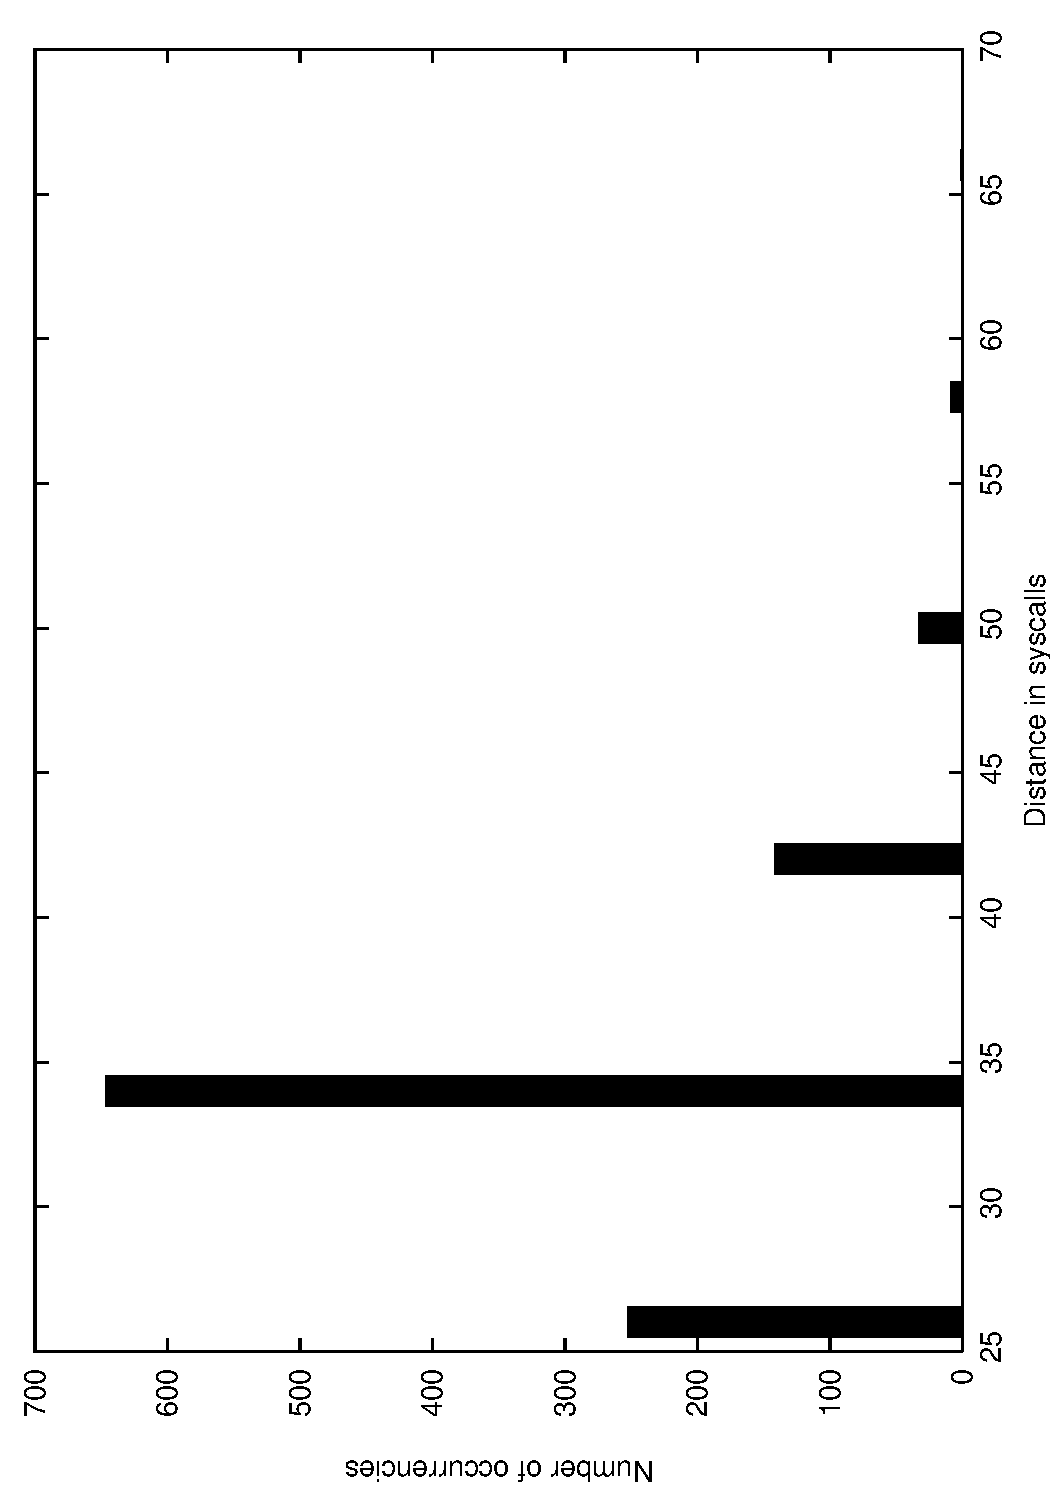
\includegraphics[angle=-90,width=.8\textwidth]{Figures/telnet.pdf}
\caption{\texttt{telnetd}: distribution of the number of other system calls among two \texttt{execve} system calls (i.e., distance between two consecutive \texttt{execve}).}
\label{fig:exectelnet}
\end{figure}

%------------------------------------------------

\section{Bulleted List}

\begin{itemize}
\item $O = $``Intrusion'', $\neg O =$``Non-intrusion'';
\item $A = $``Alert reported'', $\neg A =$``No alert reported''.
\end{itemize}

%------------------------------------------------

\section{Numbered List}

\begin{enumerate}
\item $O = $``Intrusion'', $\neg O =$``Non-intrusion'';
\item $A = $``Alert reported'', $\neg A =$``No alert reported''.
\end{enumerate}

%------------------------------------------------

\section{A Description}

\begin{description}
\item[Time] refers to the use of \emph{timestamp} information, extracted from network packets, to model normal packets. For example, normal packets may be modeled by their minimum and maximum inter-arrival time.
\item[Header] means that the \ac{TCP}\index{TCP} header is decoded and the fields are modeled. For example, normal packets may be modeled by the observed ports range.
\item[Payload] refers to the use of the payload, either at
\ac{IP}\index{IP} or \ac{TCP}\index{TCP} layer. For example, normal packets may be modeled by the most frequent byte in the observed payloads.
\item[Stochastic] means that stochastic techniques are exploited to create models. For example, the model of normal packets may be constructed by estimating the sample mean and variance of certain features (e.g., port number, content length).
\item[Deterministic] means that certain features are modeled following a deterministic approach. For example, normal packets may be only those containing a specified set of values for the \ac{TTL}\index{TTL} field.
\item[Clustering] refers to the use of clustering (and subsequent classification) techniques. For instance, payload byte vectors may be compressed using a \ac{SOM} where class of different packets will stimulate neighbor nodes.
\end{description}

%------------------------------------------------

\section{An Equation}

\begin{equation}
d_a(i,j) := \left\{
\begin{array}{lll}
K_a + \alpha_{a} \delta_{a}(i,j) & \mbox{if the elements are different} \\
0 & \mbox{otherwise}
\end{array}
\right.
\label{eq:distfunction}
\end{equation}

%------------------------------------------------

\section{A Theorem, Proposition \& Proof}

\begin{thm}
$a^2 + b^2 = c^2$
\end{thm}

\begin{prop}
$3 + 3 = 6$
\end{prop}

\begin{proof}
For any finite set $\{p_1,p_2,...,p_n\}$ of primes, consider $m = p_1p_2...p_n+1$. If $m$ is prime it is not in the set since $m > p_i$ for all $i$. If $m$ is not prime it has a prime divisor $p$. If $p$ is one of the $p_i$ then $p$ is a divisor of $p_1p_2...p_n$ and hence is a divisor of $(m - p_1p_2...p_n) = 1$, which is impossible; so $p$ is not in the set. Hence a finite set $\{p_1,p_2,...,p_n\}$ cannot be the collection of all primes.
\end{proof}

%------------------------------------------------

\section{Definition}

\begin{definition}[Anomaly-based \ac{IDS}]
An \emph{anomaly-based \ac{IDS}} is a type of \ac{IDS} that generate alerts $\mathbb{A}$ by relying on normal activity profiles.
\end{definition}

%------------------------------------------------

\section{A Remark}

\begin{rem}
Although the network stack implementation may vary from system to system (e.g., \textsf{Windows} and \textsf{Cisco} platforms have different implementation of \ac{TCP}).
\end{rem}

%------------------------------------------------

\section{An Example}

\begin{example}[Misuse \emph{vs.} Anomaly]\label{ex:misuse-vs-anomaly}
A misuse-based system $M$ and an anomaly-based system $A$ process the same log containing a full dump of the system calls invoked by the kernel of an audited machine. Log entries are in the form:

\begin{center}\small
\begin{verbatim} <function_name>(<arg1_value>, <arg2_value>, ...)
\end{verbatim}
\end{center}
\end{example}

%------------------------------------------------

\section{Note}

\begin{note}[Inspection layer]\label{note:network-stack-standardized}
Although the network stack implementation may vary from system to system (e.g., \textsf{Windows} and \textsf{Cisco} platforms have different implementation of \ac{TCP}), it is important to underline that the notion of IP, TCP, HTTP \emph{packet} is well defined in a system-agnostic way, while the notion of \emph{operating system activity} is rather vague and by no means standardized.
\end{note}
 % Include the first content chapter
%\include{Chapters/chapter2} % Include the second content chapter
%\include{Chapters/chapter3} % Include the third content chapter

\backmatter

\chapterstyle{default} % Reset the chapter style back to the default used for non-content chapters

%----------------------------------------------------------------------------------------
%	BIBLIOGRAPHY
%----------------------------------------------------------------------------------------

\bibliographystyle{plainnat} % Use the plainnat bibliography style

\bibliography{bibliography} % Use the bibliography.bib file as the source of references

%----------------------------------------------------------------------------------------
%	INDEX
%----------------------------------------------------------------------------------------

\printindex % Print the index

%----------------------------------------------------------------------------------------

\end{document}